\chapter{Side-channel attacks}

	\begin{figure}
		\begin{center}
			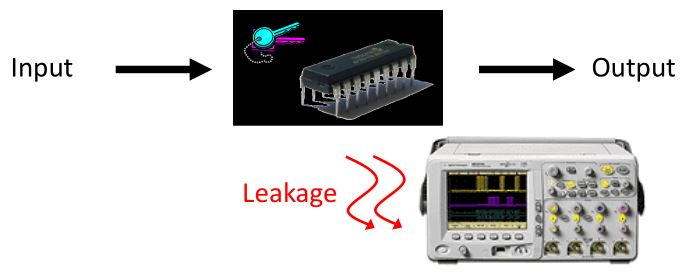
\includegraphics[scale=.6]{sideChannelLeakage}
			\caption{Esempio di side-channel attack}
			\label{fig:attack}
		\end{center}
	\end{figure}
	
	In figura [\ref{fig:attack}] si può vedere una configurazione tipo di side-channel attack. Da una parte c'è il dispositivo che implementa la funzione crittografica e accanto c'è lo strumento utilizzato per rilevare le grandezze fisiche prodotte dal dispositivo attaccato. La cosa fondamentale è che questo tipo di attacchi non vanno a colpire direttamente la funzione crittografica ma sfruttano le informazioni dell'ambiente intorno al dispositivo.